\section{L2 Switch Controller}
% \subsection{Overview}
In Experiment 3, we confirm the operation of the L2 switch. The L2 switch is an OSI two-layer MAC address-based network device that forwards frames to destinations to improve the defects of the HUB that cause bottlenecks.The operation of the L2 switch is as follows as example between h1 and h3:
\vspace{-3mm}
\begin{enumerate}
    \item Send packets from Host h1 to Host h3
    \item \textbf{Learning-1} : Store the MAC address and port number of the origin h1 Host in the MAC table
    \item \textbf{Flooding} : Destination h3 Host's MAC address is not in the MAC table, so it is sent to all ports
    \item Send packets to Host h1 using MAC address received from flooding from Host h3
    \item \textbf{Learning-2} : Store the origin MAC address and port number (Host h3) in the MAC Rable in process 4
    \item \textbf{Forwarding} : Prior to the process 5, the MAC table has only the MAC address and port number of Host h1, the first sender, so only the stored Host h1 can be transferred by h3 (h3 → h1 forwarding)
\end{enumerate}
\vspace{-3mm}
In the following experiment, we are going to compare the flow table before and after transmission of the packet to check how the example between h1 and h3's process proceeds.
\vspace{-1.5mm}
\subsection{Flow table before sending the packet}
\vspace{-4mm}
\begin{figure}[!h]\centering 
	\includegraphics[width=.99\textwidth]{image/week06/3-1-1.png}
	\caption{\footnotesize 
	Terminal out screenshot : Flow table with activating forwarding L2 switch}
	\vspace{-10pt}
\end{figure}
\clearpage
\subsection{Sending Packet : Ping test results (H1 $\to$ H3)}
\begin{figure}[!h]\centering 
	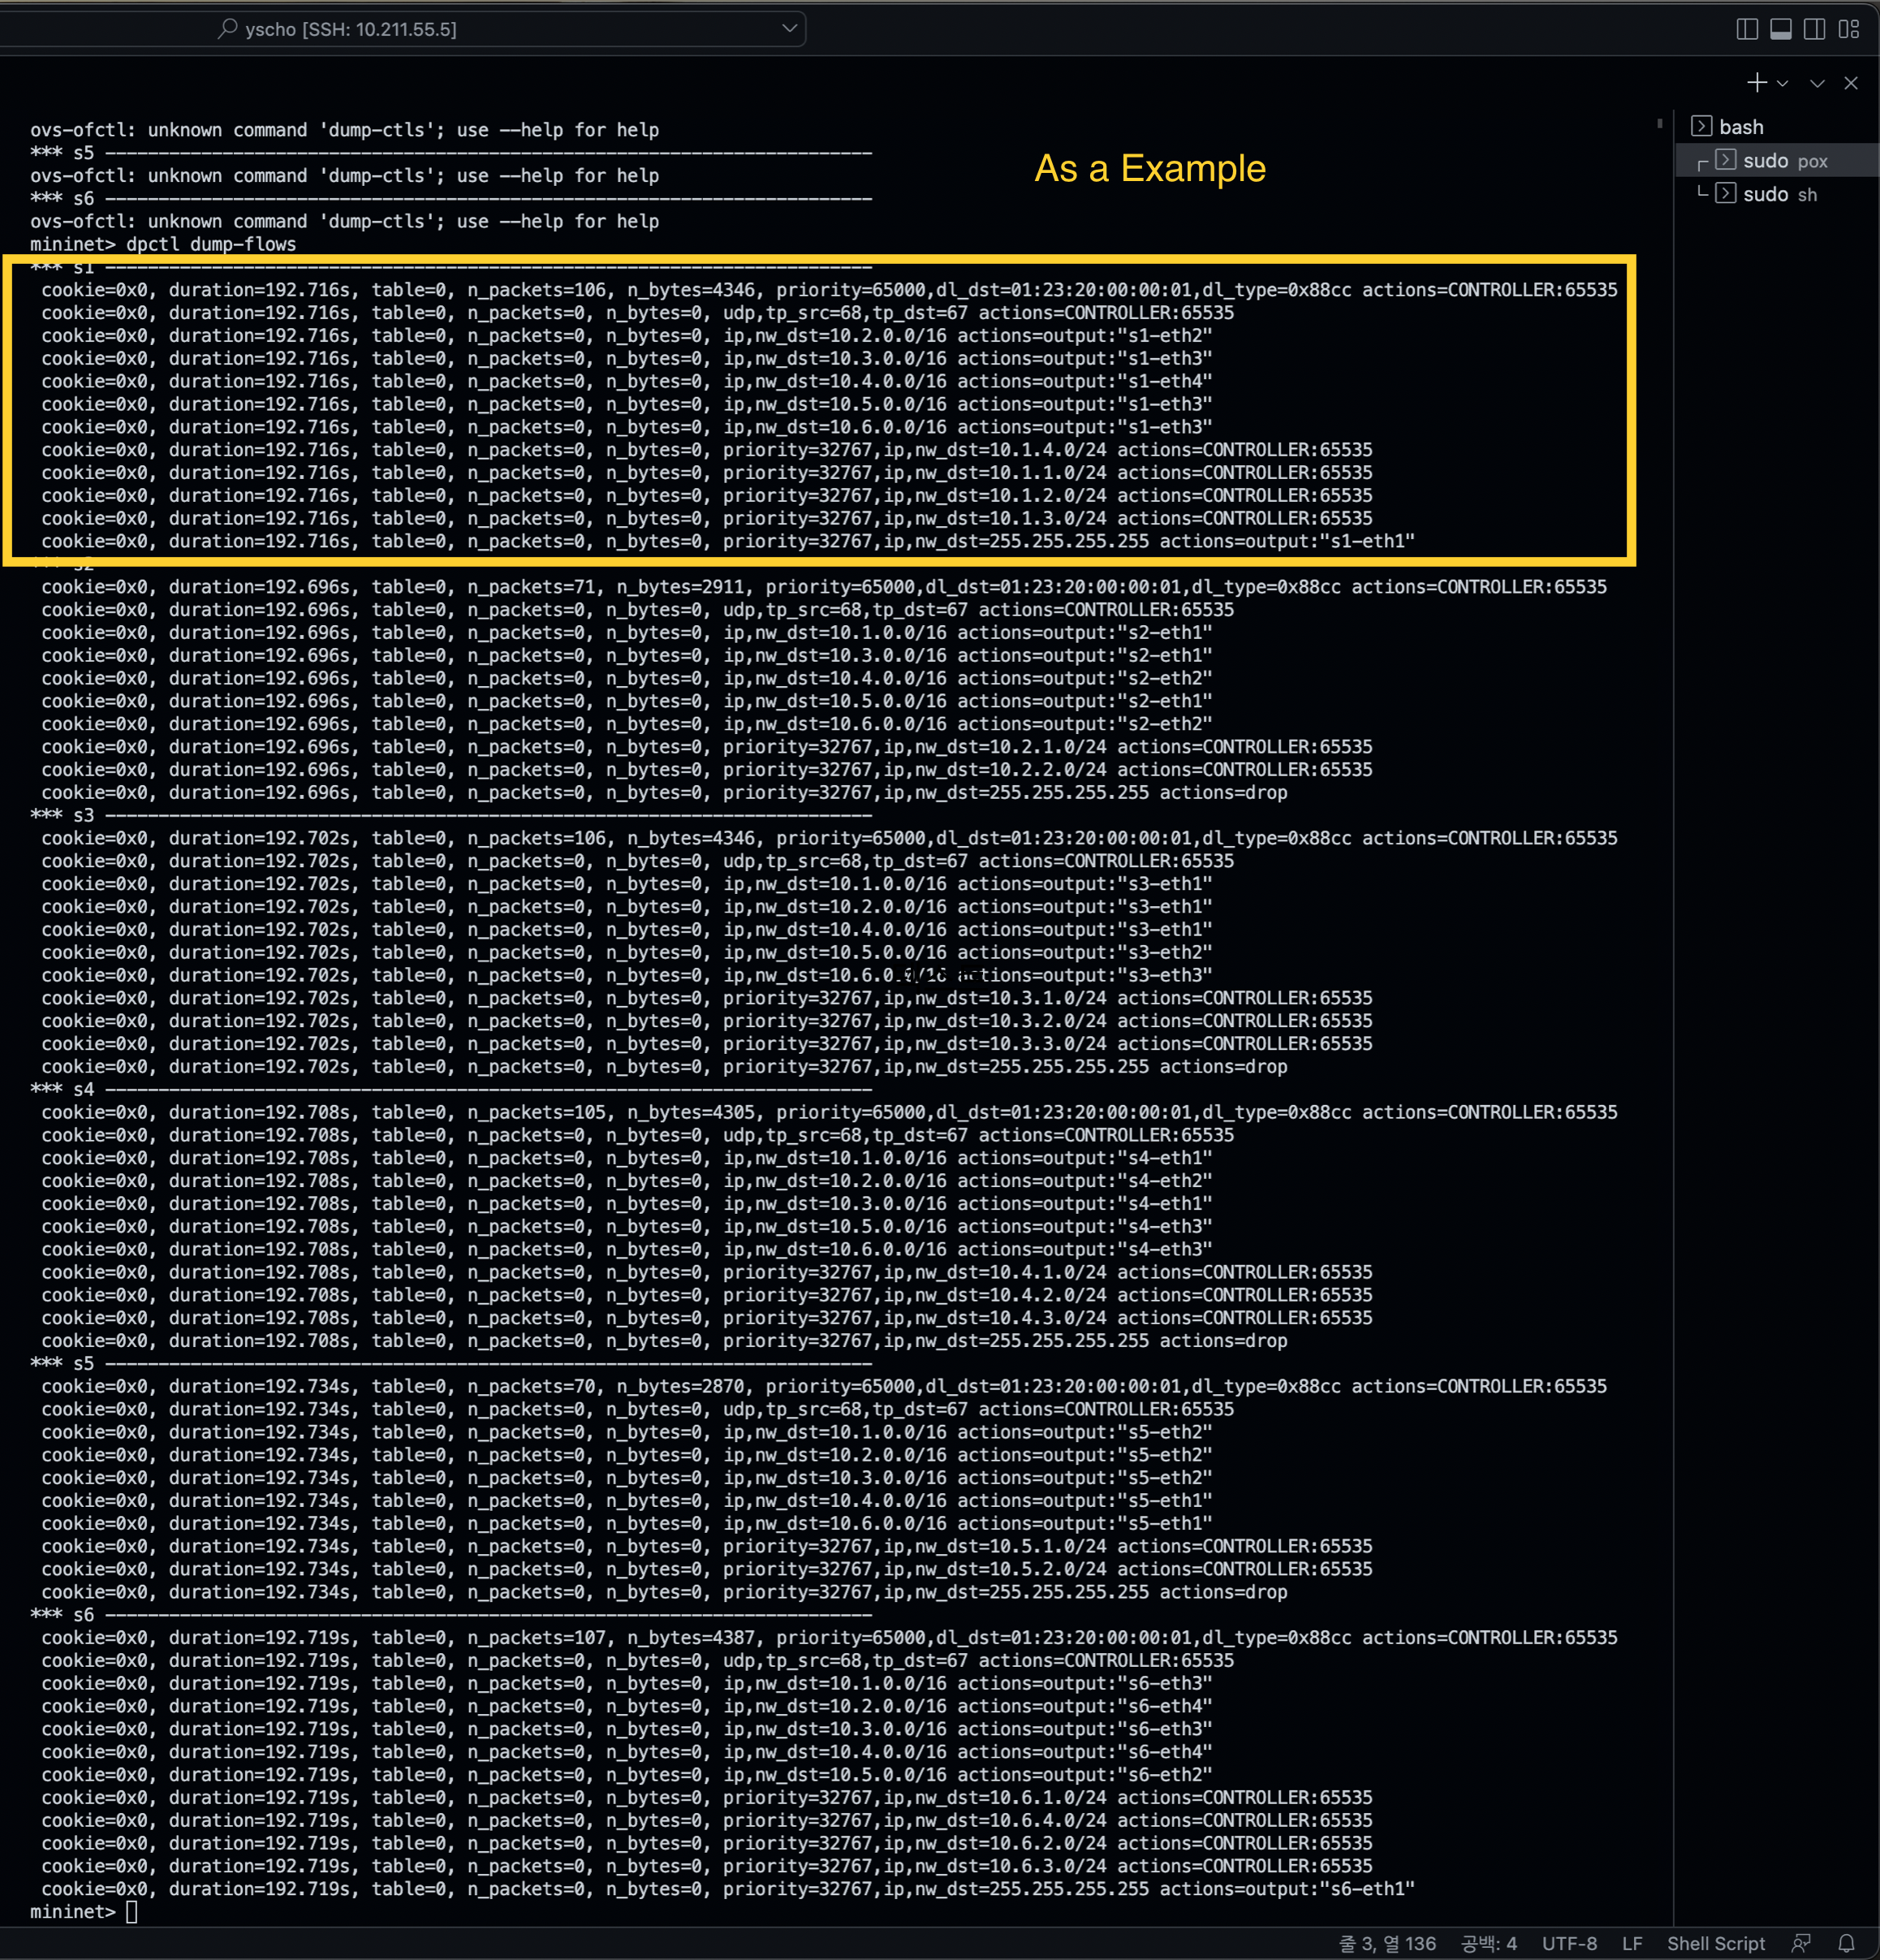
\includegraphics[width=.99\textwidth]{image/week06/3-1.png}
	\caption{\footnotesize 
	Terminal out screenshot : Sending the two packets (h1 $\to$ h3)}
	\vspace{-10pt}
\end{figure}
\subsection{Flow table after sending the packet}
In the figure we can find out the 2 of learing processes that updates the MAC Table adding the MAC addtrss of h1 and h3 in first four log line and then forwarding process that sends packet from h3 to h1 in last fifth log line.\\
\vspace{-4mm}
\begin{figure}[!h]\centering 
	\includegraphics[width=.99\textwidth]{image/week06/3-2.png}
	\caption{\footnotesize 
	Terminal out screenshot : Flow table with activating forwarding L2 Switch}
	\vspace{-10pt}
\end{figure}
\subsubsection*{Discussion}
In the previous example, when transmitting a packet from Host h1 to Host h3, the process of forwarding the L2 switch was checked based on the change in the MAC table.

Through the learning process between h1 and h3 corresponding to stage 2 and 5, the results in which the forwarding corresponding to stage 6 is from h3 to h1 may be confirmed through the flow table after sending the packet.
\subsection{Interface Listening}
The detailed process of packets exchanged between h1 and h3 could be confirmed by interface listening experiment.\\
As the previous series of example shows, in the case of h2 the only once transmission of packets in flooding process that is to learn the address of h3 in h1 while they change the packet in forwding that of after learning process.
\clearpage
\vspace{-4mm}
\begin{figure}[h!]
\centering
\subfloat[Screenshot of h1's terminal]{
    \includegraphics[width=0.33\textwidth]{image/week06/3-3-1.png}
}
\subfloat[Screenshot of h2's terminal]{
    \includegraphics[width=0.33\textwidth]{image/week06/3-3-2.png}
}
\subfloat[Screenshot of h3's terminal]{
    \includegraphics[width=0.33\textwidth]{image/week06/3-3-3.png}
}\caption{Terminal out screenshot : Each host's interaface terminal}
\end{figure}
\vspace{-8mm}
\subsection{Throughput test}
\begin{figure}[h!]
\centering
\captionsetup[subfloat]{labelformat=empty}
\subfloat[$N = 3$ : 80.2, 80.4 Gbits / sec]{
    \includegraphics[width=0.95\textwidth]{image/week06/3-4-1.png}
}\hfill
\subfloat[$N = 30$ : 84.8, 85.0 Gbits / sec]{
    \includegraphics[width=0.95\textwidth]{image/week06/3-4-2.png}
}\hfill
\subfloat[$N = 300$ : 73.6, 73.7 Gbits / sec]{
    \includegraphics[width=0.95\textwidth]{image/week06/3-4-3.png}
}
\end{figure}
\clearpage
\subsubsection*{Discussion}
Unlike Hubs, L2 switches do not force bandwidth allocation per host because the flooding action of transmitting throughout the connected host is performed only in the first case of adding an address to the MAC table.

However, the slight decrease in bandwidth as the number of hosts increases is considered to the possibility of collision in the first flooding step is proportional increasing to the number of hosts.
\clearpage